\chapter{Related Works}

%\section{Parallel Imaging}
%"Self-Calibrating Nonlinear Reconstruction Algorithms for Variable Density Sampling and Parallel Reception MRI" by Loubna El Gueddari, C. Lazarus, H Carrié, A. Vignaud, Ph Ciuciu

%SENSE and ESPIRiT for sensitivity map estimation

\color{red}
This chapter contains the text I copied from the project reports I've done with Wièm and Mahmoud, but this is far from ready!
\color{black}

\subsection{Sparse Formulation}


"Compressed Sensing MRI" (2008) by Michael Lustig, David L. Donoho, Juan M. Santos, and John M. Pauly --> "A look at how CS can improve on current imaging techniques"

"Sparse MRI: The Application of Compressed Sensing for Rapid MR Imaging" (2007) by Michael Lustig, David Donoho, and John M. Pauly

Having the measurement data that exhibit a required level of sparsity and incoherence, makes us able to apply optimization methods to reconstruct the original image from that undersampled measurement. The optimization problem is formulated in the following way: $$\textit{minimize} \lvert\lvert \Psi m \rvert\rvert_1 \textit{ such that } \lvert\lvert \mathcal{F}_u m - y \rvert\rvert_2 < \epsilon,$$
where $m$ image of interest, $\Psi$ a sparsifying transform, $\mathcal{F}_u$ undersampled Fourier transform, $y$ measured k-space data, $\epsilon$ threshold for expected noise level (controls fidelity of reconstruction). Minimizing $\lvert\lvert \Psi m \rvert\rvert_1$ promotes sparsity, constraint $\lvert\lvert \mathcal{F}_u m - y \rvert\rvert_2 < \epsilon$ enforces data consistency. When $\Psi$ is finite-differences operator (difference of neighbors), then we refer to $\lvert\lvert \Psi m \rvert\rvert_1$ as $TV(m)$. That operator is used many times as additional penalty: \textit{minimize} $\lvert\lvert \Psi m \rvert\rvert_1 + \alpha TV(m)$ \textit{such that} $\lvert\lvert \mathcal{F}_u m - y \rvert\rvert_2 < \epsilon$ where $\alpha$ trades $\Psi$ sparsity with finite-differences sparsity. Although there exist multiple methods to solve that constrained optimization problem, constrained optimization problems are considered to be difficult tasks to solve, so most of the times researchers try to find a way to convert the problem to unconstrained formulation. In our case, the Lagrangian form is a good solution to that problem:
$$\argmin_m \lvert\lvert\mathcal{F}_u m - y \rvert\rvert_2^2 + \lambda \lvert\lvert\Psi m \rvert\rvert_1,$$
where $\lambda$ is a regularization parameter that determines the trade-off between data consistency and sparsity. if $\lambda$ properly selected, then the two problem statements yield same results. $\lambda$ can be determined by trying many values and choosing one so that $\lvert\lvert\mathcal{F}_u m - y \rvert\rvert_2 \approx \epsilon$. Adding the total variance term and introducing the $f$ function to note the cost function, we get the following formula:
$$\argmin_m f(m)$$
$$\text{ where } f(m) := \lvert\lvert\mathcal{F}_u m - y \rvert\rvert_2^2 + \lambda \lvert\lvert\Psi m \rvert\rvert_1 + \alpha TV(m).$$

After these modifications, we can find many methods to minimize $f$ efficiently:
\begin{itemize}
    \item interior point methods
    \item projections onto convex sets
    \item homotopy
    \item iterative soft thresholding
    \item iteratively reweighted least squares
    \item nonlinear conjugate gradients (used in that article)
\end{itemize}
In the following, we attempt to briefly explain the motivation behind the \textit{nonlinear conjugate gradient} method, and show its mechanism.

\paragraph{Transform Sparsity}
 Sparse signals are signals that have a few non zero coefficients. Most natural signals like images and sounds are compressible i.e. can be represented with few nonzero coefficients in a certain basis without a big loss of information. While MR images are sparse in discrete cosine transform (DCT) and wavelet transform domains, angiograms, for instance, have already a sparse pixel representation.  One famous sparsifying transform is the Spatial Finite Differences which consists in computing the difference between neighboring pixels so the only non zero values are those of the pixels at the edges. Dynamic MR images are also highly compressible and have a sparse representation in the temporal Fourier Domain~\cite{parrish, lustig}.
 
\subsection{Incoherence of Artifacts}
Since a complete sampling of the k-space is a time-consuming process, only a subset is generally acquired by MRI scanners. Due to the sparse nature of the original signal, the latter can still be recovered from a small number of measurements. However, due to the violation of the Nyquist criterion, undersampling in the frequency domain results in aliasing artifacts. In the case of equidistant undersampling, the artifacts are coherent which makes it difficult to reconstruct the signal. For an intuitive visualization, see fig.~\ref{fig:incoherence}. However, taking random samples results in incoherent artifacts that behave like additive noise.
Truly random sampling in the k-space is generally impractical due to hardware and physiological constraints. The sampling must follow smooth lines and curves and be robust to real-life situations. Several sampling trajectories exist and can be seen in Fig.~\ref{fig:trajectories}.


\begin{figure}
    \centering
    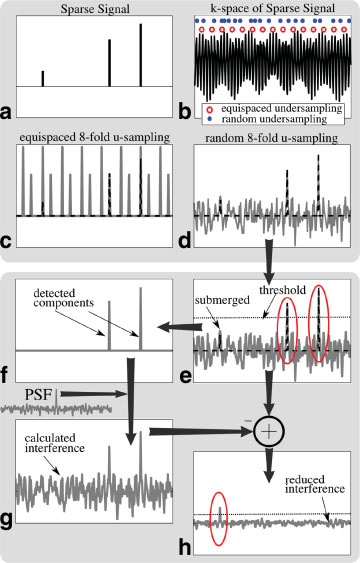
\includegraphics[width=\linewidth]{images/project with Wiem/fig-001.png}
    \caption{An intuitive reconstruction of a sparse signal from pseudo-random k-space undersampling. A sparse signal (a) is 8-fold undersampled in k -space (b). Equispaced undersampling results incoherent signal aliasing (c) that cannot be recovered. Pseudo-random undersampling results in incoherent aliasing (c). Strong signal components stick above the interference, are detected (e) and recovered (f) by thresholding. The interference of these components is computed (g) and subtracted (h), lowering the total interference level and enabling recovery of weaker components. Image and caption from~\cite{sparse}.}
    \label{fig:incoherence}
\end{figure}

\subsubsection{Measuring Coherence} 
In the following we introduce two tools to measure the coherence between samples: 
Point Spread Function (PSF) and Transform Point Spread Function (TPSF).
\begin{itemize}
    \item Point Spread Function (PSF):
    $$PSF(i,j)=e_{j}^{*}F_{u}^{*}F_{u}e_{i}$$
    measures contribution of a unit-intensity pixel at the $i^{th}$ position to a pixel at $j^{th}$ position  
    \item Transform Point Spread Function (TPSF):
    $$TPSF(i,j)=e_{j}^{*}\Psi F_{u}^{*}\Psi_{*} F_{u}e_{i}$$
    measures influence of a single transform
    coefficient to other transform coefficients. Here $F_{u}$ is the undersampled Fourier Operator, $\Psi$ is an orthogonal sparsifying matrix, $e_{i}$ and $e_{j}$ are basis vectors.
\end{itemize}
\begin{figure}
    \centering
    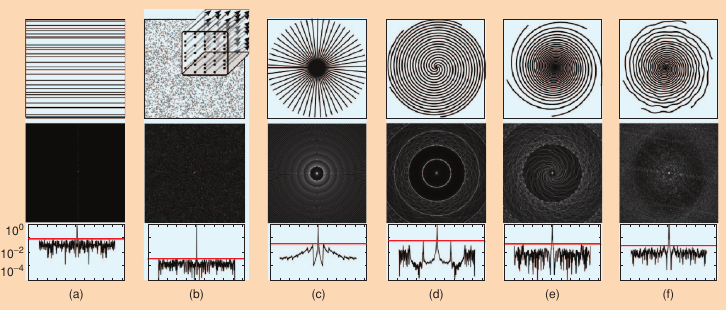
\includegraphics[width=\linewidth]{images/project with Wiem/non-cartesian-sampling.png}
    \caption{PSFs of various sampling trajectories: (a) random lines in 2-D, (b) random points in 2-D or cross-section of random lines in 3-D, (c) radial, (d) uniform spirals, (e) variable density spirals, and (f) variable density perturbed spirals. The height of the red lines measures coherence. Image and caption from~\cite{compressed}.}
    \label{fig:trajectories}
\end{figure}

\subsubsection{Variable Density Random Undersampling}
Our incoherence analysis assumes nonzero elements scattered randomly in the k-space in a sparse representation.  However, in natural images, most of the energy is concentrated around the origin of the k-space.
A uniform random distribution of samples in the spatial-frequency domain does not
take into account the energy distribution of MR images in k-space.   Therefore it makes more sense to opt for a nonuniform variable
density sampling matching energy distribution in k-space. Precisely, we should consider having more samples from the central part of the frequency domain and less highfrequency components. One possibility is sampling with density scaling according to a power of distance from the origin. Fig.~\ref{fig:trajectories} shows examples of physically feasible sampling patterns.

\section{Proximal Optimized Gradient Method}
Why is it faster than FISTA, and why is it optimal

D. Kim and J. A. Fessler, “Optimized first-order methods for smooth convex minimization,” Math. Program., vol. 159, no. 1, pp. 81–107, Sep. 2016, doi: 10.1007/s10107-015-0949-3.

\section{Decompositions}

\subsection{Low rank and Sparse}
C. Y. Lin and J. A. Fessler, “Efficient Dynamic Parallel MRI Reconstruction for the Low-Rank Plus Sparse Model,” IEEE Transactions on Computational Imaging, vol. 5, no. 1, pp. 17–26, Mar. 2019, doi: 10.1109/TCI.2018.2882089.

J. A. Fessler, “Optimization methods for MR image reconstruction (long version),” arXiv:1903.03510 [eess, math], Jun. 2019.

\subsection{Multiscale}

Ong's dissertation: “Low Dimensional Methods for High Dimensional Magnetic Resonance Imaging,” 2018.

F. Ong et al., “Extreme MRI: Large-Scale Volumetric Dynamic Imaging from Continuous Non-Gated Acquisitions,” arXiv:1909.13482 [physics], Dec. 2019.

Differences between Ong's dissertation and his "extreme MRI" preprint paper

\section{IRSL}
Iteratively reweighted Least Squares method

C. Kümmerle and C. M. Verdun, “Denoising and Completion of Structured Low-Rank Matrices via Iteratively Reweighted Least Squares,” arXiv:1811.07472 [cs, math], Nov. 2018.

Henry Adams, Lara Kassab, and Deanna Needell "An Iterative Method for Structured Matrix Completion"

\clearpage % You need \clearpage at the end of every chapter to force images included in this chapter to be rendered in somewhere else